% Appendix B. GNURadio Companion
%==========================================================================

\chapter{GNURadio Companion}
\label{AppB}

\emph{GNURadio} incluye una aplicaci\'on que facilita el desarrollo de grafos y aplicaciones
sencillas de manera gr\'afica, muy similar al software de Simulink de Mathworks. La aplicaci\'on
genera codigo en Python apartir del diagrama de bloques que uno define. Es posible manipular y
extender el codigo generado si es que se desea utilizar alguna funci\'on que no este incluida en
\emph{GNURadio Companion}\cite{grc} (GRC por sus siglas en ingles). Las capacidades de la
aplicaci\'on son:

\begin{itemize}
  \item Viene incluido con el codigo fuente de \gnuradio. Si se instalan todas las dependencias
  entonces GRC se instalar\'a junto con \gnuradio.
  \item Puede generar codigo en Python para aplicaciones que utilizan bloques graficos con la
  libreria WxWidgets, aplicaci\'ones que no utilizan ningun control grafico y bloques jer\'arquicos.
  \item Se pueden definir bloques que actuan como variables o constantes. Otros bloques pueden hacer
  referencia a ellas e incluir su valor en algun par\'ametro. Tambien es posible usar bloques
  variables que definen un control grafico como barras deslizadoras, botones, etc.
  \item Cada bloque esta definido por un archivo XML que contiene todas sus caracteristicas (numero
  de puertos, tipo de datos con los que trabja, par\'ametros de entrada, etc.). Es posible crear un
  archivo XML para incluir algun bloque creado por el usuario.
  \item Los bloques pueden ser deshabilitados dentro de la gr\'afica sin tener que borrarlos de la
  aplicaci\'on. Estos bloques son ignorados por el generador de codigo, permitiendo asi una manera
  mas rapida de realizar cambios en la gr\'afica. Tambien se pueden cortar, copiar y pegar bloques.
\end{itemize}

Para poder instalar GRC se deben de tener las siguientes dependencias intaladas antes de iniciar la
compilaci\'on:

\begin{itemize}
  \item Python 2.5 o mayor (\url{http://www.python.org/download/})
  \item Python-LXML 2.0 o  mayor (\url{http://codespeak.net/lxml/installation.html})
  \item Cheetah Template Engine 2.0 o mayor (\url{http://www.cheetahtemplate.org/download.html})
  \item Python-GTK 2.10 o mayor (\url{http://www.pygtk.org/downloads.html})
\end{itemize}

Si estas dependencias se instalan antes de iniciar con la compilaci\'on de \gnuradio entonces GRC se
instalar\'a autom\'aticamente.

Para iniciar la aplicaci\'on se necesita abrir una ventana de consola y escribir el comando
\verb|gnuradio-companion|. Inmediatamente aparecer\'a la ventana que se muestra en la figura
\ref{fig:grc}.

\begin{figure}[tp]
  \centering
  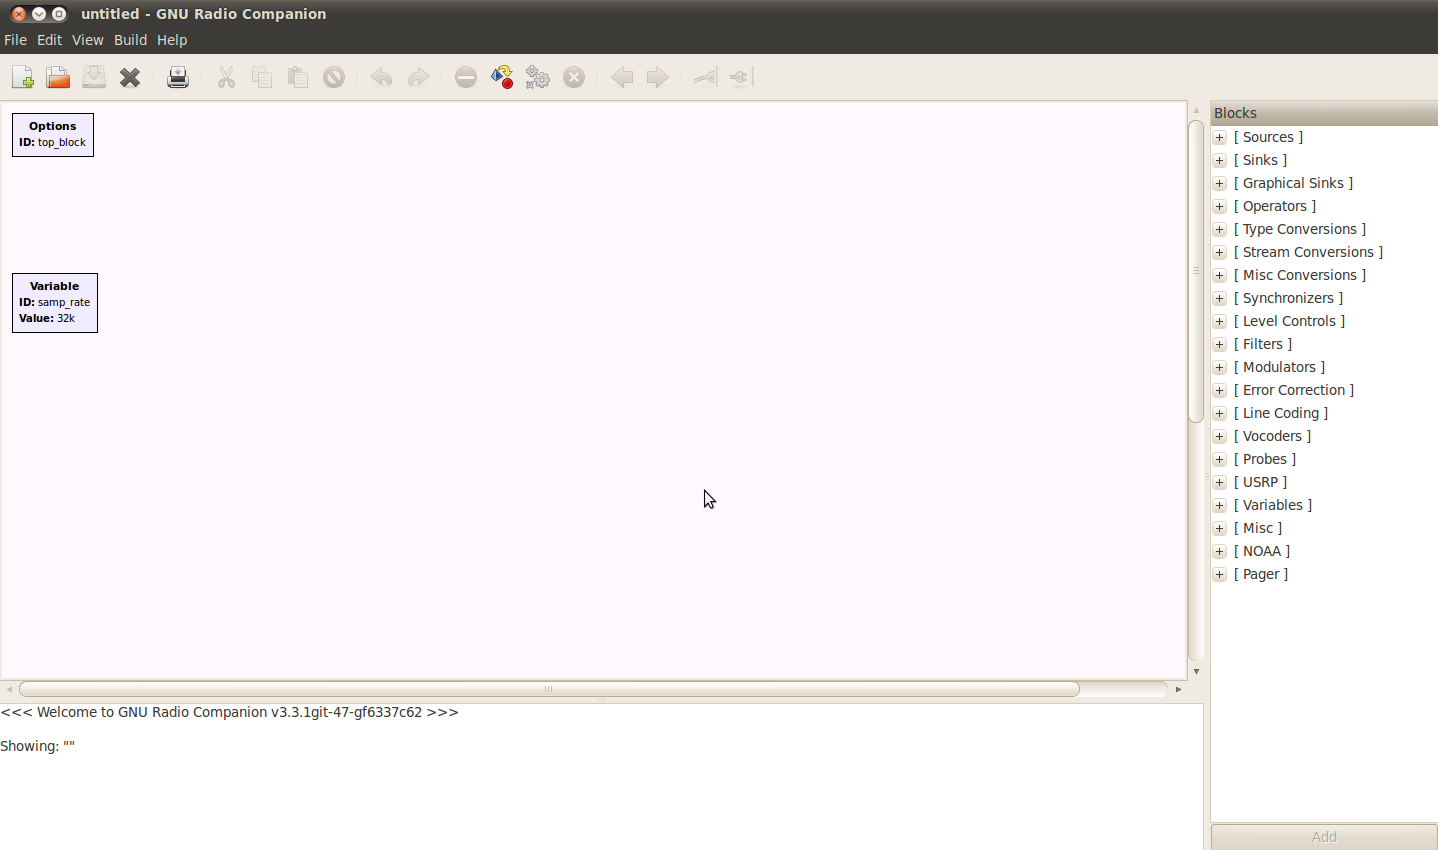
\includegraphics[width=5.5in]{figs/grc1}
  \vspace{0.3in}
  \caption{Pantalla principal de GNURadio Companion}
  \label{fig:grc}
\end{figure}

La \'area de trabajo inicia con dos bloques por default, uno que define las opciones generales del
grafo y un bloque que define una variable llamada \verb|sample_time|. Esta variable se puede
modificar o borrar seg\'un las necesidades del usuario. Del lado derecho se encuentra la lista de las
categor\'ias de bloques que soporta GRC. Cada categor\'ia se puede expandir para revelar los
diferentes bloques que contiene. Para colocar bloques en el \'area de trabajo es necesario
seleccionar el de inter\'es y arrastrarlo con el mouse a la area de trabajo. De ahi se puede seguir
arrastrando para colocarlo en el \'area que el usuario desee. 

Las propiedades de los bloques se pueden obtener haciendo doble click sobre el bloque como se
muestra en la figura \ref{fig:blockprop}.

\begin{figure}[tp]
  \centering
  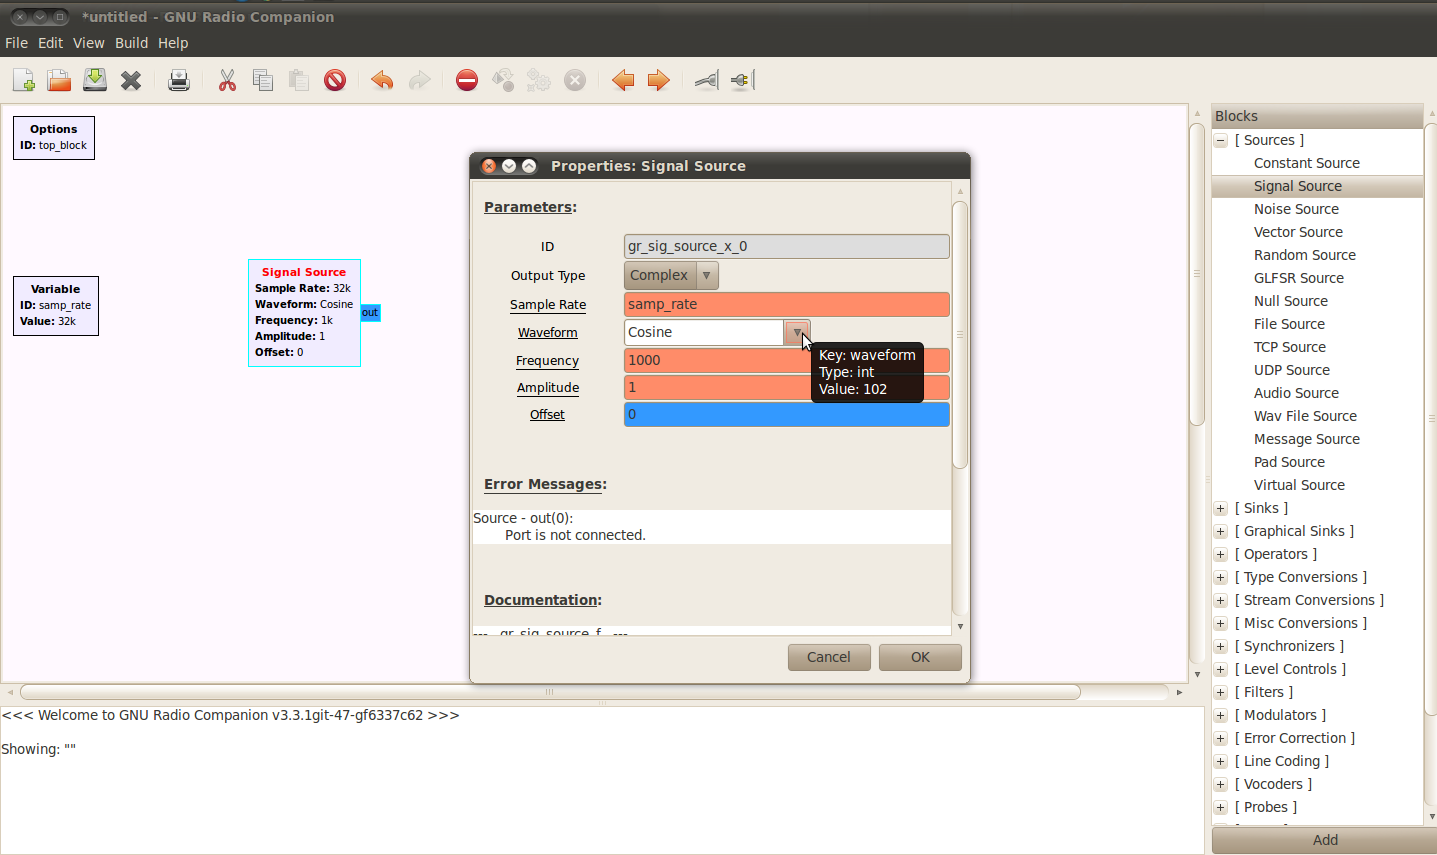
\includegraphics[width=5.5in]{figs/grc3}
  \vspace{0.3in}
  \caption{Pantalla de propiedades del bloque signal\_source}
  \label{fig:blockprop}
\end{figure}

Todos los bloques comparten un parametro en comun y es el ID. Este parametro indentifica al bloque
para que otros puedan hacer referencia a el. Se puede aceptar el nombre default que GRC sugiere o
bien se puede especificar otro. Los otros par\'ametros son especificos del bloque con el que se esta
trabajando. EL bloque \verb|signal_source| de la figura \ref{fig:blockprop} es un generador de
se\~nales que puede generar varios tipos de formas de onda como senoidales, cuadradas, dientes de
sierra, etc. Los par\'ametros se describen como sigue:

\begin{description}
\item[Output Type] Especifica el tipo de datos que se va utilizar: Real o Complejo.
\item[Sample Rate] La taza de muestreo con la que se generar\'a la se\~nal. Aqui se muestra haciendo
referencia al bloque que declara la variable \verb|sample_rate|. Esta variable tiene un valor de
32k.
\item[Waveform] Aqui se define el tipo de se\~nal que se quiere generar.
\item[Frequency] Este parametro especifica la frecuencia de la se\~nal.
\item[Amplitude] Este parametro especifica la amplitud de la se\~nal.
\item[Offset] Especifica un retraso de la se\~nal generada.
\end{description}

En la figura \ref{fig:grcex} muestra un ejemplo completo de un grafo que suma dos se\~nales de
diferentes frecuencias y muestra el resultado en un osciloscopio.

\begin{figure}[tp]
  \centering
  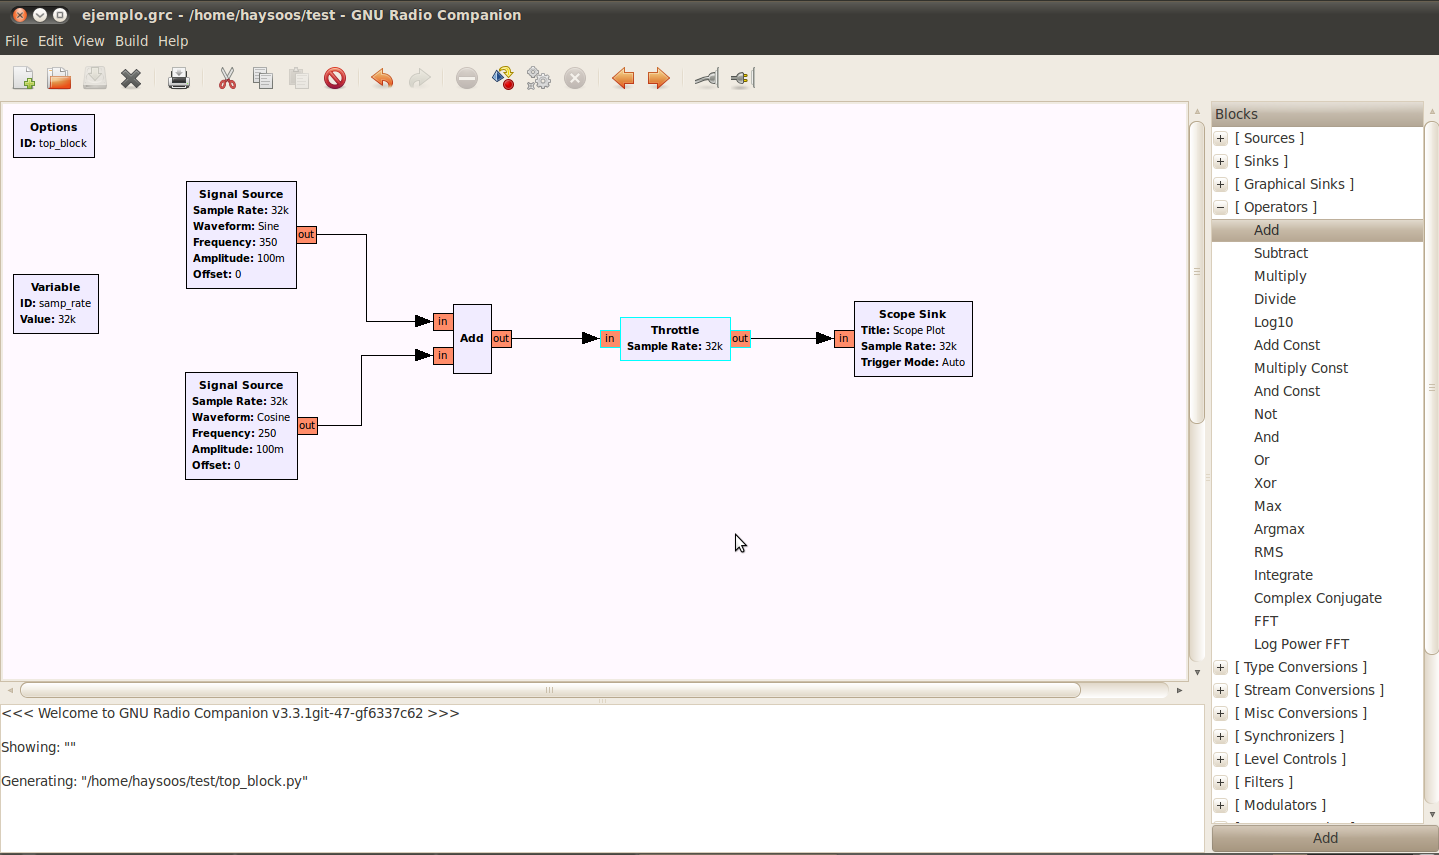
\includegraphics[width=5.5in]{figs/grc6}
  \vspace{0.3in}
  \caption{Ejemplo de un grafo desarrollado en GRC}
  \label{fig:grcex}
\end{figure}

El ejemplo muestra un requerimiento importante de los grafos que no utilizan fuentes o sinks de
hardware como el USRP o la tarjeta de sonido. Los bloques que hacen referencia a algun hardware
limitan autom\'aticamente la velocidad de ejecuci\'on del grafo a la velocidad de muestreo del
hardware. Como el ejemplo de la figura \ref{fig:grcex} no contiene este tipo de bloques es
necesario incluir el bloque \verb|Throttle| para limitar la velocidad de ejecuci\'on, de lo
contrario el grafo se ejecutar\'a a la velocidad m\'axima del CPU y esto causara que la PC no
responda correctamente. Para este ejemplo el bloque hace referencia a la variable \verb|sample_rate|
declarada y con esto limita la velocidad de ejecuci\'on a la taza de muestreo que se esta utilizando.

El bloque \verb|Scope Sink| es uno de los diversos visualizadores graficos que permiten observar las
se\~nales en diversos puntos del grafo. Este bloque actua como un osciloscopio con opciones de
disparo y modo XY. Otros bloques con los que cuenta GRC para visualizar se\~nales son: analizador de
espectros, espectrograma en 2D, histograma y diagrama de constelaci\'on.

Si existe un error en alguna de las conexiones, ya sea porque los tipos de datos son incompatibles
entre bloques, algunas de las opciones no est\'an correctamente configuradas o falta alg\'un puerto
por conectar, estos ser\'an enfatizados de color rojo. Es necesario realizar las correcciones que se
piden antes de generar el c\'odigo y poder ejecutar el grafo.

%TODO: Get the name of the run buttons
Para ejecutar el grafo es necesario hacer click en el boton de generar codigo o en el de ejecutar
grafo. Si no se ha grabado el trabajo GRC pedir\'a que se grabe antes de la ejecuci\'on como se
muestra en la figura \ref{fig:savegrc}. Una vez realizado esto GRC genera un archivo con codigo
Python y este es el que se ejecuta. La figura \ref{fig:rungrc} muestra el grafo de la suma de las
dos se\~nales ejecutandose y mostrando los resultados en un osciloscopio.

\begin{figure}[htp]
  \centering
  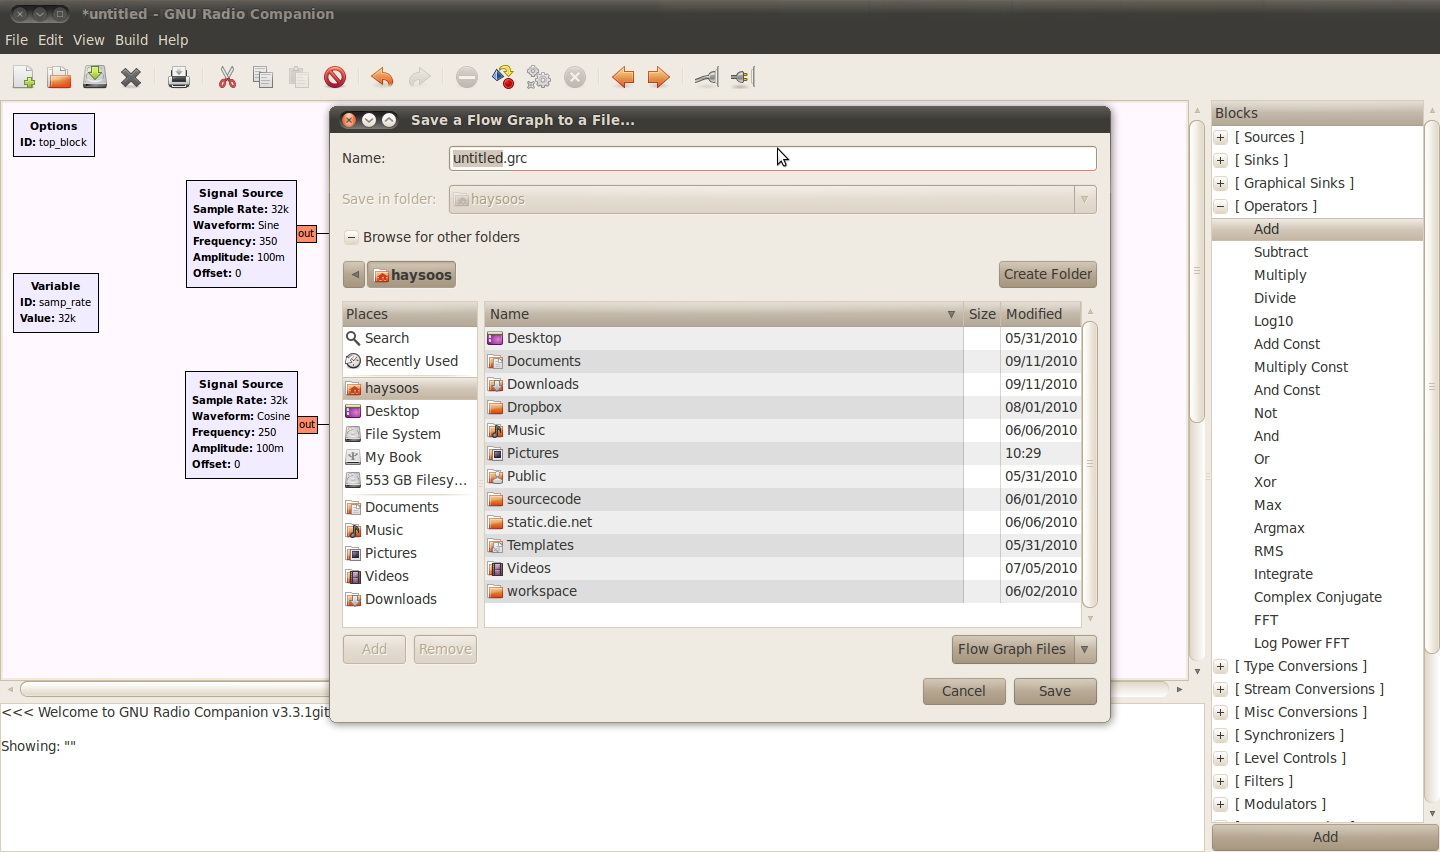
\includegraphics[width=5.5in]{figs/grc5}
  \vspace{0.3in}
  \caption{Pantalla para salvar el trabajo en GRC}
  \label{fig:savegrc}
\end{figure}

\begin{figure}[htp]
  \centering
  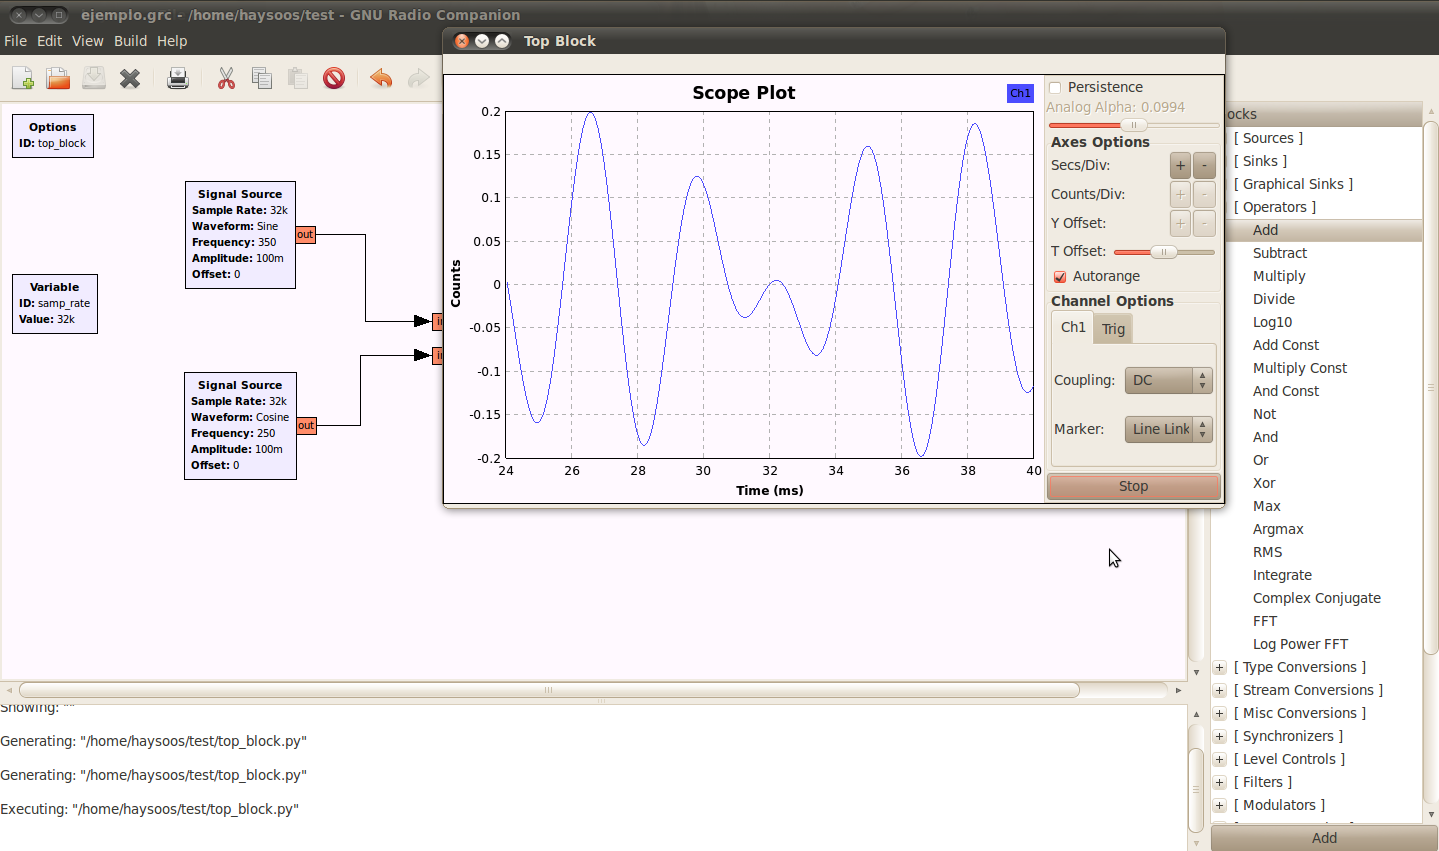
\includegraphics[width=5.5in]{figs/grc7}
  \vspace{0.3in}
  \caption{Ejemplo de un grafo en ejecuci\'on}
  \label{fig:rungrc}
\end{figure}

Conforme se vallan anexando bloques visualizadores estos se van agrupando en la misma pantalla de
forma vertical. Esto permite visualizar los resultados de una manera m\'as eficiente sin tener que
estar cambiando entre diferentes ventanas. Agregando el bloque FFT al ejemplo obtenemos la pantalla
que se muestra en la figura \ref{fig:fftgrc}.

\begin{figure}[htp]
  \centering
  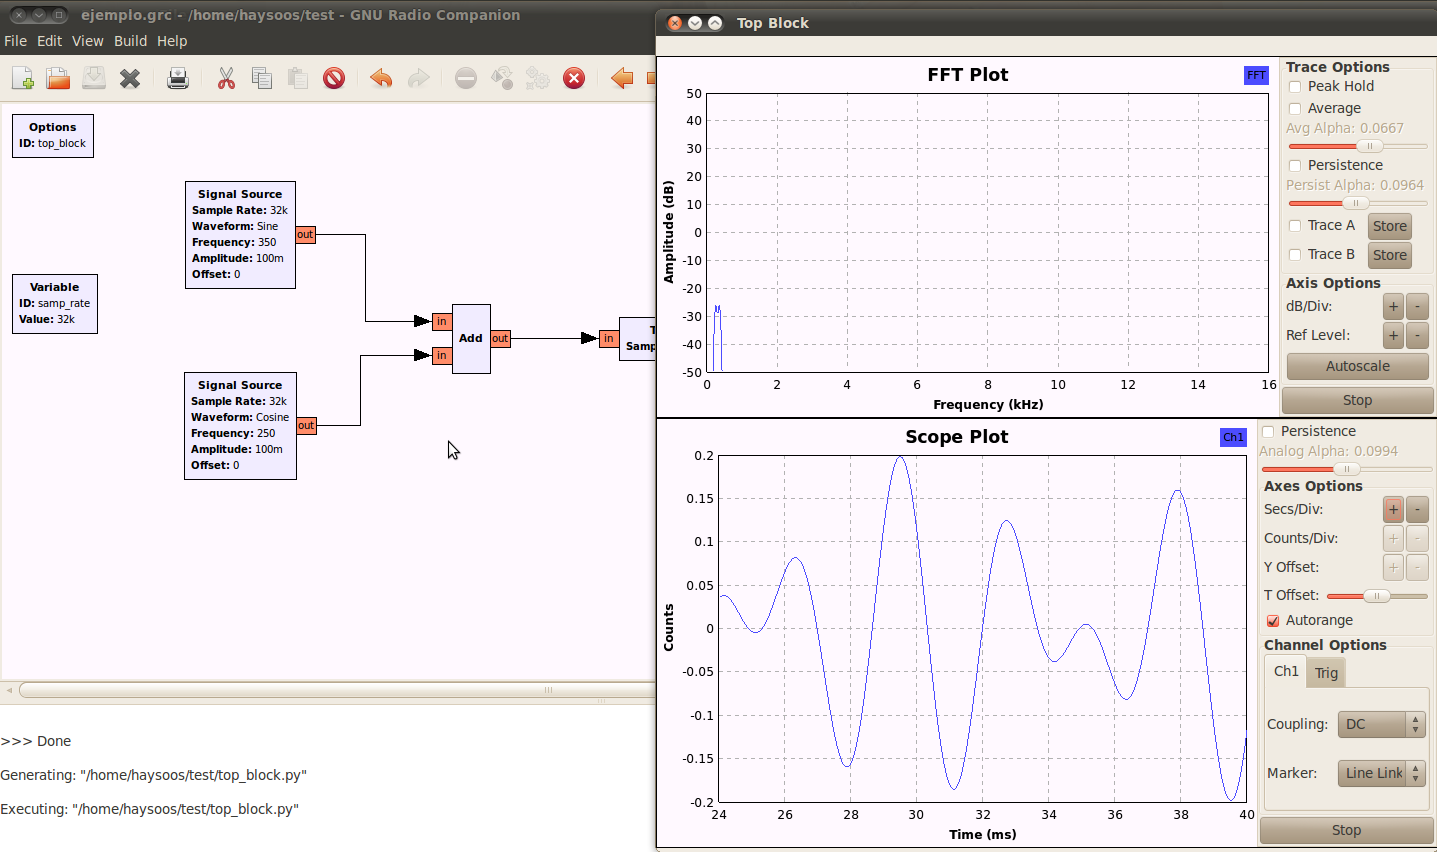
\includegraphics[width=5.5in]{figs/grc8}
  \vspace{0.3in}
  \caption{Bloque FFT en conjunto con el osciloscopio en GRC}
  \label{fig:fftgrc}
\end{figure}

Como se menciono al inicio de este ap\'endice, una de las habilidades de GRC es poder especificar
bloques que implementan alg\'un tipo de control grafico como barras deslizadoras. Estos controles se
anexan autom\'aticamente junto con los otros controles gr\'aficos y act\'uan como un bloque con
algun valor variable que puede modificar cualquier par\'ametro del grafo. Para ilustrar esto al
ejemplo se anexa un bloque de este tipo con el nombre de amplitud. Al bloque se le especifica un valor default,
valor m\'aximo y m\'inimo y el tipo de dato con el que trabaja. Asignando esta variable a los campos
de amplitud de los dos bloques \verb|Signal Source| se puede modificar la amplitud de ambos moviendo la
barra deslizadora que aparece en la ventana de visualizaci\'on como se muestra en la figura
\ref{fig:vargrc}.

\begin{figure}[htp]
  \centering
  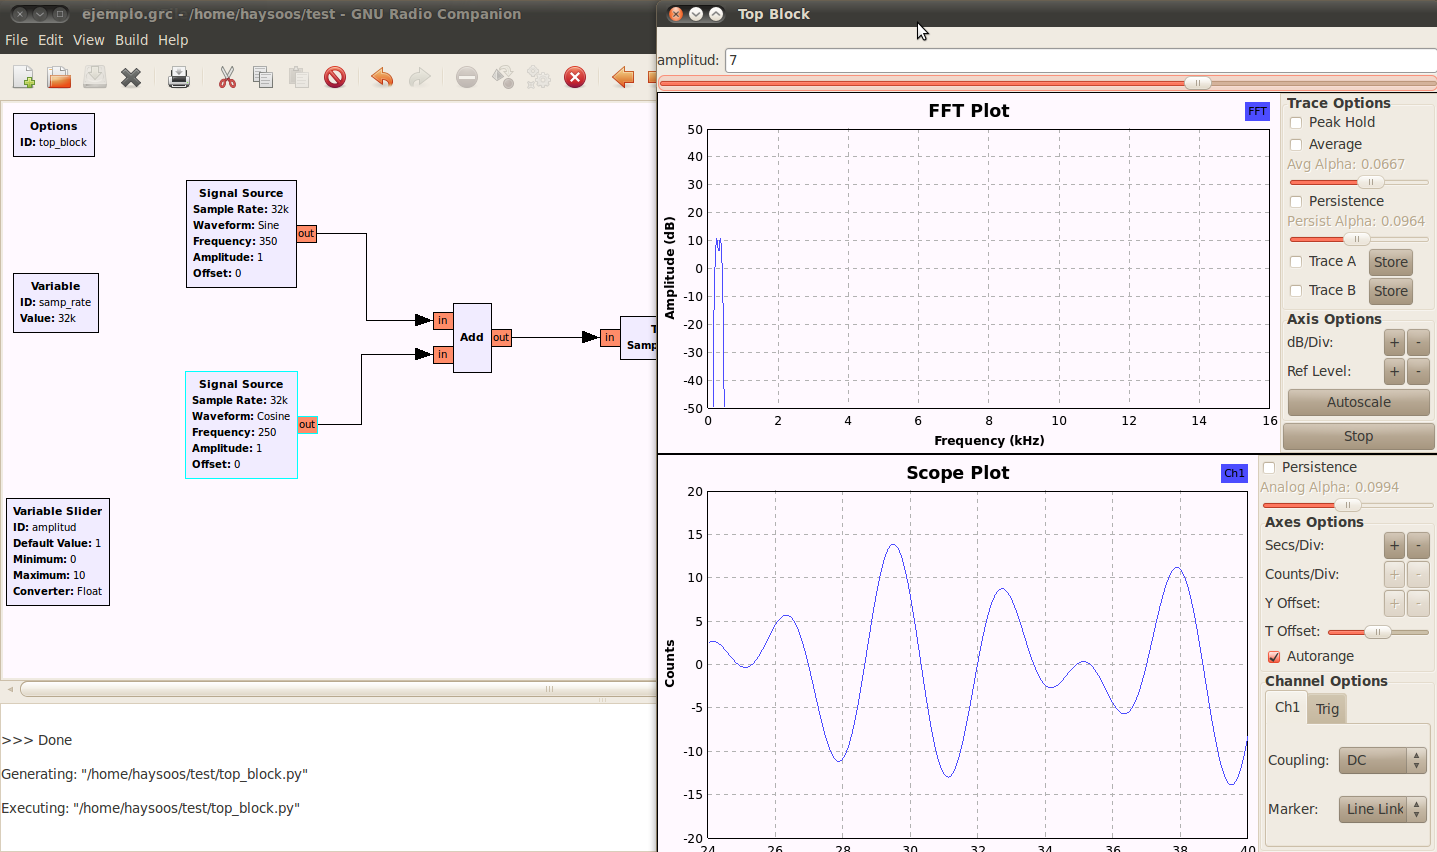
\includegraphics[width=5.5in]{figs/grc9}
  \vspace{0.3in}
  \caption{Modificaci\'on de par\'ametros por medio de bloques variables en GRC}
  \label{fig:vargrc}
\end{figure}

El ejemplo ilustrado en este ap\'endice es un solo un peque\~na ilustraci\'on de las capacidades de
\emph{GNURadio Companion}. Los bloques de los generadores de se\~nales se pueden remplazar por
bloques que encapsulan alg\'un hardware como tarjetas de audio, el USRP o incluso tarjetas de
adquisici\'on de datos, aunque para estas es necesario crear el bloque desde cero y proporcionar los
drivers del hardware adecuados. Tambi\'en es posible trabajar con varios filtros como pasa bajas,
hilbert y ventanas. GRC en si act\'ua como una interfaz gr\'afica a los bloques de \gnuradio
facilitando as\'i su uso de una manera m\'as intuitiva. Esto permite una mejor interacci\'on con el
software para aplicaciones acad\'emicas donde la experiencia con programaci\'on no es necesaria.
